\section{Problem Formulation}
\label{sec:problem}

\paragraph{Setting.}
A prompt is a pair $(q, C)$: a question $q$ written on the user side and an excerpt $C$
drawn from an IoT log. The excerpt is split into units $U(C)=\{u_1,\dots,u_m\}$, one per
record or key--value group. Each case carries a set of protected values
$V=\{v_1,\dots,v_n\}$; a unit is \emph{sensitive} when it contains a value in $V$. A model
$M$ answers $q$ from the compressed context, and the answer is scored against a reference
span.

\paragraph{What must not reach the model.}
The prompt is the object of study. It travels from the device to the model process and may
be logged, cached, or inspected. A policy is \emph{leak-free} on a case when no value in $V$
is recoverable from the exact text handed to the model, that is, from the rewritten question
$q'$ concatenated with the compressed context, not from the context alone. Recoverability is
measured with the pattern set of the published protocol (full value plus fragments). We
assume no adversarial manipulation of the model and no side channel beyond the prompt text,
and we do not model an adversary who holds the alias map; Section~\ref{sec:discussion}
states what that leaves out.

Figure~\ref{fig:concept} fixes three things that the rest of the paper depends on. Panel~(a)
is the reason the operation matters: the answer text is identical in all three rows, and only
the first column separates a value that can still be addressed from one that cannot. Deleting a
sensitive unit keeps the answer and destroys the statement of whose answer it is, which is why
redaction and routing are not two settings of one knob. Panel~(b) is the boundary the privacy
claim is written against: the prompt is the only thing that crosses, the alias map stays on the
operator's side, and the three adversaries at the bottom have very different reach. Panel~(c)
is the plane we report in: a compressor moves along the frontier, buying utility with privacy,
and the corner where both are high is empty. Our argument is that reaching it is a change of
operation rather than a better point on that curve.

\begin{figure*}[t]
\centering
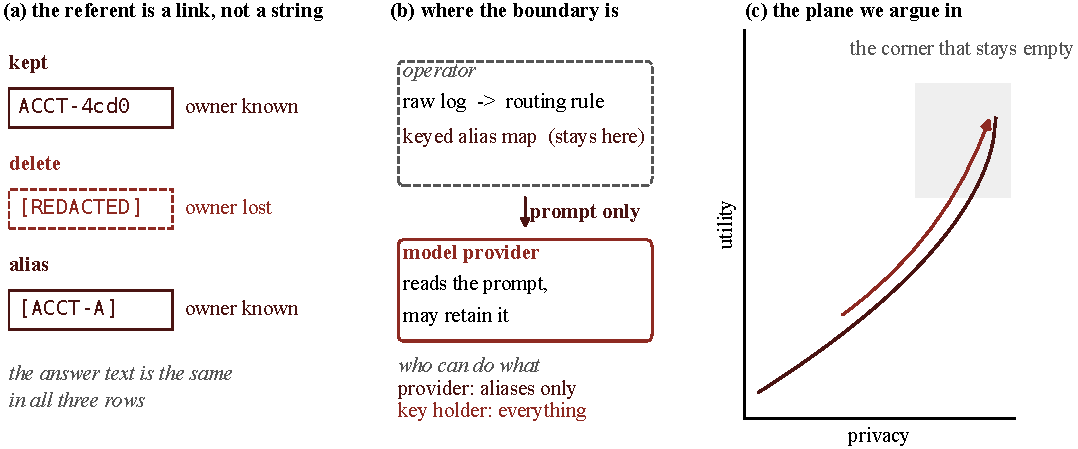
\includegraphics[width=\textwidth]{figures/fig_concept.pdf}
\caption{The three premises of the evaluation. (a)~The referent is a link, not a string: all
three rows carry the same answer text, and only the first column decides whether the reader can
tell which record it belongs to. Deletion produces the second row, aliasing the third; the
answer survives either way, so an endpoint that measures only the answer cannot see the
difference. (b)~What crosses the trust boundary: the prompt only, with the keyed alias map
retained by the operator. The three adversaries named at the bottom differ in what they can
reach, and the privacy claim is stated against the first of them. (c)~The plane the results live
in, drawn conceptually here and measured in Figure~\ref{fig:frontier}. Compression today trades
one axis for the other along the curve; the shaded corner is where both are high, and it is
empty for every method that moves along that curve.}
\label{fig:concept}
\end{figure*}

\paragraph{The queried entity.}
Each question names an entity $e^\star$, which may be an account, a device, or a record
identifier. The \emph{anchor} $A\subseteq U(C)$ is the set of units containing a mention of
$e^\star$. A unit plays a referential role when the question cannot be resolved without
knowing which entity a value belongs to.

\paragraph{Budget.}
A budget arm receives a ratio $r$ and must realise a compressed context of at most
$B=\lceil r\cdot n_C\rceil$ tokens, where $n_C$ is the token length of the uncompressed
excerpt under the tokenizer used to build the prompt. Exceeding $B$ is a hard error rather
than a silent truncation, because in this domain the answer region is often at the end of the
excerpt and truncation would remove it without notice.

\paragraph{Metrics.}
\begin{itemize}
\item \textbf{Task quality.} EM and F1 from the standard SQuAD~v2 scorer;
\textsc{unknown} is not a legal answer.
\item \textbf{Prompt leak}. Fraction of cases in which any protected value is recoverable
from question plus compressed context. Lower is better.
\item \textbf{Gold-in-context (GIC)}. Fraction of cases in which the reference span survives
compression. It is model-free, and therefore an upper bound on what the reader can achieve;
it is also blind to whether the surviving span is still interpretable, which is why we report
task quality as a separate endpoint.
\item \textbf{Referential integrity}. A case satisfies it when three conditions hold together:
the answer span survives ($A_s$), distinct entities do not collapse onto one surface token
($E_c$), and the handle in the question names the same entity as the handle in the context
($M_r$). We write $RI=A_s\cdot E_c\cdot M_r$, a conjunction rather than a score, because the
task needs all three and none substitutes for another. Table~\ref{tab:ri} measures each factor
and shows why the conjunction is the right form: two configurations zero exactly one factor and
both lose the task, while the configuration that keeps all three is the only one that also
answers it. We report the three factors separately alongside $RI$ so that a zero can be
attributed; a product that hid which factor failed would be uninformative here, since the
failures have different remedies.
\item \textbf{Overshoot}. Indicator that a budget arm exceeded $B$ on a case.
\end{itemize}

\begin{table}[t]
\caption{Referential integrity and its three factors, measured on the same $2{,}728$ cases.
\emph{$A_s$}: the answer span survives. \emph{$E_c$}: distinct entities do not collapse onto one
surface token. \emph{$M_r$}: the alias in the question and the alias in the context name the
same entity. $RI$ is the conjunction, $A_s\cdot E_c\cdot M_r$, because the task needs all three
and each one alone is not enough. Two configurations zero exactly one factor and both lose the
task; the row that keeps all three is the only one that also answers it. $RI$ is necessary, not
sufficient---the uncompressed arm and \textsc{DARK} both score $100$ and still differ in F1,
which is why the two endpoints are reported separately.}
\label{tab:ri}
\centering\small
\setlength{\tabcolsep}{4pt}
\resizebox{\columnwidth}{!}{%
\begin{tabular}{lrrrrr}
\toprule
Configuration & $A_s$ & $E_c$ & $M_r$ & $RI$ & F1 \\
\midrule
uncompressed                        & 100.00 & 100.00 & 100 & 100 & 0.6081 \\
\textbf{\textsc{DARK}}              & \textbf{100.00} & \textbf{100.00} & \textbf{100} & \textbf{100} & \textbf{0.4937} \\
\quad alias replaced by delete      & 100.00 &   0.00 & 100 &   0 & 0.3142 \\
\quad question not rewritten        & 100.00 & 100.00 &   0 &   0 & 0.3132 \\
anchor line kept                    &  57.55 & 100.00 & 100 &  57.55 & 0.3352 \\
global alias                        &  57.59 & 100.00 & 100 &  57.59 & 0.3482 \\
\bottomrule
\end{tabular}}
\end{table}


\paragraph{The condition we study.}
The setting is narrow and we state it as such: long, identifier-dense operational text; a
question that names an entity; and a requirement that the entity's value not reach the
model. Questions of this form are common in IoT operations and, as
Section~\ref{sec:analysis} shows, are exactly the ones on which redundancy-based compression
is harmful. The same routing reduces to ordinary compression when the question is topical
and names no entity; we report that variant as out of scope rather than as a success.
